\subsection{Graphics}
According to requirement \ref{graphicsReq}, the graphics must be kept simple.
To accommodate this both the background and the objects have been kept simple and two dimensional.
The graphics used in the game can be seen on \cref{pausedstate}.
The background of the game is kept simple.
The road is a simple grey texture, and there is a border of grass in the top and the bottom of the screen, consisting of a green texture.

\begin{figure}[h]
\begin{subfigure}{0.5\textwidth}
\centering

\includegraphics{car}
\caption{The car}
\label{car}
\end{subfigure}
~
\begin{subfigure}{0.5\textwidth}
\centering

\includegraphics{obstacle}
\caption{An obstacle}
\label{obstacle}
\end{subfigure}

\begin{subfigure}{\textwidth}
\centering
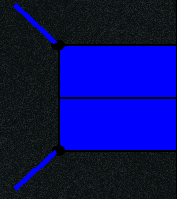
\includegraphics{garage}
\caption{One of the garages}
\label{garage}
\end{subfigure}
\caption{The graphics used in the game}
\label{graphicszoom}
\end{figure}

The individual objects can be seen on \cref{graphicszoom}.
The graphics are chosen so they are simple and yet recognizable.